\documentclass[10pt]{beamer}

\usepackage[T2A]{fontenc}
\usepackage[utf8]{inputenc}
\usepackage[russian,english]{babel}

\usefonttheme[onlymath]{serif}

\usetheme[progressbar=frametitle]{metropolis}
\usepackage{appendixnumberbeamer}

\usepackage{booktabs}
\usepackage[scale=2]{ccicons}

\usepackage{pgfplots}
\usepgfplotslibrary{dateplot}

\usepackage{xspace}
\newcommand{\themename}{\textbf{\textsc{metropolis}}\xspace}
\newcommand{\TODO}[1]{\textbf{\textcolor{red}{TODO: #1}}}

\date{}
\author{Екатерина Тузова}


\title{Лекция 6}
\subtitle{Перцептрон}

\begin{document}

\maketitle

\section{Разбор летучки}

\section{Мотивирующий пример}

\begin{frame}\frametitle{Пример}
  \TODO{пример}  
\end{frame}

\begin{frame}\frametitle{Пример}
  \alert{Идея}: Назначим каждому признаку объекта некоторый вес. Посчитаем взвешенную сумму и если она больше некоторого порогового значения, отнесем объект к искомому классу. 
\end{frame}

\begin{frame}\frametitle{Модель McCulloch-Pitts}
  $X$ - множество объектов \\
	$Y$ - множество классов \\
	\pause
	$$a(x,w) = \sigma(\sum\limits_{j=1}^n w_j f_j(x) - w_0) = \sigma(\langle w, x \rangle)$$\\
  $f_j$ — числовые признаки, $j = 1,\dots, n$ \\	
	$w_j \in R$ -- веса признаков\\
	$\sigma(s)$ -- функция активации (например, $\sign$)
	\pause
	\begin{figure}[htbp]
	  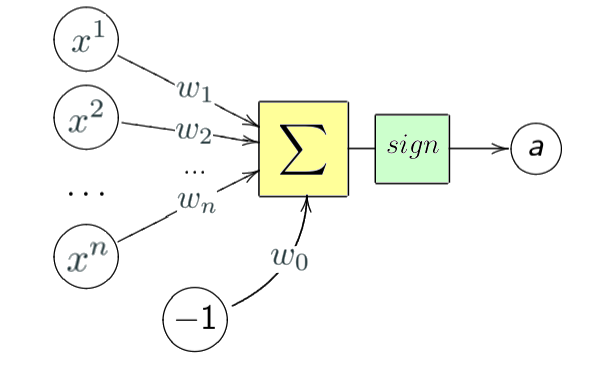
\includegraphics[height=100pt, keepaspectratio = true]{images/neuron-scheme}   
	\end{figure}
\end{frame}

\begin{frame}{Алгоритм}
	\begin{algorithmic}[1]
        \Function{perceptron}{$X$, $\eta$}
            \State Инициализировать ${w_0, \dots, w_n}$
            \MRepeat [пока $w$ изменяются] 
               \For {$i = 1, \dots, n$}
                 \State $w = w - \eta (a(x_i) - y_i) x_i$
               \EndFor
           	\EndRepeat
        \EndFunction
    \end{algorithmic}
\end{frame}


\begin{frame}\frametitle{Линейные алгоритмы классификации и регрессии}
	Задача классификации: \\
	$Y = \left\{ \pm1 \right\}, \hspace{10mm} a(x,w) = \sign \langle w, x_i \rangle $\\
	$Q(w;X^l) = \sum\limits_{i=1}^l \mathcal{L} (\langle w, x_i\rangle y_i) \rightarrow \min\limits_w$\\
	\bigbreak
	\pause
	Задача регрессии:\\
	$Y = \mathbb{R}, \hspace{10mm} a(x,w) = \sigma(\langle w, x_i \rangle)$\\
	$Q(w;X^l) = \sum\limits_{i=1}^l (\sigma(\langle w, x_i \rangle) - y_i)^2 \rightarrow \min\limits_w $
\end{frame}

\section{Какой класс функций можно реализовать нейроном?}

\begin{frame}\frametitle{Любую ли функцию можно представить нейросетью?}
	\begin{enumerate}[--]
		\item Двухслойная сеть в $\left\{0, 1 \right\}^n$ позволяет реализовать произвольную булеву функцию.
		\item Двухслойная сеть в $\mathbb{R}^n$ позволяет отделить произвольный выпуклый многогранник.
		\item Трёхслойная сеть $\mathbb{R}^n$ позволяет отделить произвольную многогранную область, не обязательно выпуклую, и даже не обязательно связную.
		\item С помощью линейных операций и одной нелинейной функции активации $\sigma$ можно приблизить любую непрерывную функцию с любой желаемой точностью
	\end{enumerate}
\end{frame}

%\begin{frame}\frametitle{Регрессия}
%	$X$ -- объекты в $\mathbb{R}^n$ 
%	$Y$ -- ответы в $\mathbb{R}$\\
%	$X^l = (x_i, y_i)_{i=1}^l$ -- обучающая выборка\\
%	$y : X \rightarrow Y$ -- неизвестная зависимость\\
%  \pause	
%	\vspace{5mm}
%	$a(x) = f (x, w)$ -- модель зависимости,\\
%	$w \in \mathbb{R}^p$ -- вектор параметров модели.\\
%	\vspace{5mm}
%	\pause
%	Метод наименьших квадратов (МНК):\\
%	$$Q(w,X^l) = \sum\limits_{i=1}^l \alpha_i (f (x_i, w) - y_i)^2 \rightarrow \min\limits_{w}$$\\
%	где $\alpha_i$ -- вес, степень важности i-го объекта.\\
%	$Q(w^*,X^l)$ — остаточная сумма квадратов
%\end{frame}
%
%\begin{frame}\frametitle{Метод максимума правдоподобия}
%	Модель данных с некоррелированным гауссовским шумом:\\
%	$$y(x_i) = f (x_i, w) + \varepsilon_i, \hspace{5mm} \varepsilon_i \in N (0, \sigma_i^2), i = 1, \dots, l$$\\
%	\vspace{5mm}
%	\textbf{Вопрос}: Как выглядит плотность одномерного Гауссовского распределения?
%\end{frame}
%
%\begin{frame}\frametitle{Нормальное распределение}
%	\begin{figure}[htbp]
%	  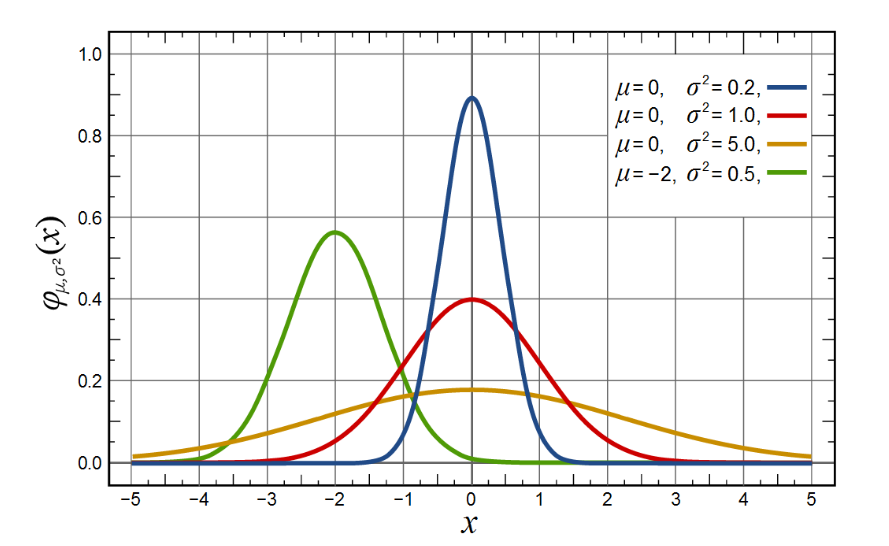
\includegraphics[height=200pt, keepaspectratio = true]{images/gauss}   
%	\end{figure}
%\end{frame}
%
%\begin{frame}\frametitle{Нормальное распределение}
%	\begin{figure}[htbp]
%	  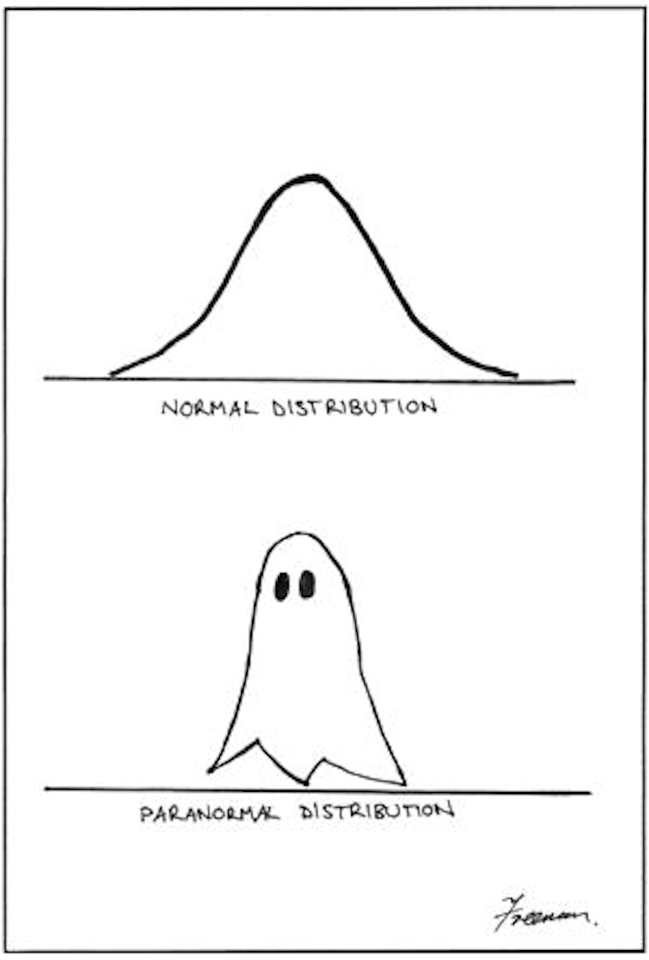
\includegraphics[height=200pt, keepaspectratio = true]{images/paranormal}   
%	\end{figure}
%\end{frame}
%
%
%\begin{frame}\frametitle{Метод максимума правдоподобия}
%	Метод максимума правдоподобия (ММП):\\
%	$$L(\varepsilon_1, \dots, \varepsilon_l | w) = \prod\limits_{i=1}^l p(\varepsilon_i) = \prod\limits_{i=1}^l \frac{1}{\sigma_i \sqrt{2\pi}} \exp (-\frac{\varepsilon_i^2}{2\sigma_i^2}  ) \rightarrow \max\limits_{w}$$\\
%	$$- \ln L(\varepsilon_1, \dots, \varepsilon_l| w) = const(w) + \frac{1}{2} \sum\limits_{i=1}^l \frac{(f(x_i, w) - y_i)^2}{\sigma_i^2}  \rightarrow \min\limits_{w}$$\\
%\end{frame}
%
%\begin{frame}\frametitle{Метод максимума правдоподобия}
%	Метод максимума правдоподобия (ММП):\\
%	$$- \ln L(\varepsilon_1, \dots, \varepsilon_l| w) = const(w) + \frac{1}{2} \sum\limits_{i=1}^l \frac{(f(x_i, w) - y_i)^2}{\sigma_i^2}  \rightarrow \min\limits_{w}$$\\
%	\vspace{2mm}
%	Метод наименьших квадратов: $$Q(w,X^l) = \sum\limits_{i=1}^l \alpha_i (f (x_i, w) - y_i)^2 \rightarrow \min\limits_{w}$$\\
%	\vspace{5mm}
%	\textbf{Удивительный факт}: Постановки МНК и ММП, совпадают, причём веса объектов
%	обратно пропорциональны дисперсии шума, $\alpha_i = \sigma_i^{-2}$
%\end{frame}
%
%\begin{frame}\frametitle{Многомерная линейная регрессия}
%	$f_1(x), \dots, f_n(x)$ -- числовые признаки\\
%	Модель многомерной линейной регрессии:\\
%	$$f (x, w) = \sum\limits_{j=1}^n w_j f_j(x), \hspace{5mm} w \in \mathbb{R}$$\\
%	\vspace{5mm}
%	Функционал квадрата ошибки:\\
%	$$Q(w,X^l) = \sum\limits_{i=1}^l (f (x_i, w) - y_i)^2  \rightarrow \min\limits_{w}$$\\
%\end{frame}
%
%\begin{frame}\frametitle{Матричное представление}
%	$$F_{l \times n} = \begin{pmatrix}
%	  f_1(x_1) & \dots & f_n(x_1) \\
%	  \dots & \dots & \dots\\
%	  f_1(x_l) & \dots & f_n(x_l)
%	 \end{pmatrix} \hspace{1mm} y_{l \times 1} = \begin{pmatrix}
%	  y_1 \\
%	  \dots\\
%	  y_l
%	 \end{pmatrix} \hspace{1mm} w_{n \times 1} = \begin{pmatrix}
%	  w_1 \\
%	  \dots\\
%	  w_n
%	 \end{pmatrix}$$ \\
%	\vspace{5mm}
%	Функционал квадрата ошибки:\\
%	$$Q(w,X^l) = \sum\limits_{i=1}^l (f (x_i, w) - y_i)^2  = \Vert Fw - y \Vert^2 \rightarrow \min\limits_{w}$$\\
%\end{frame}
%
%\begin{frame}\frametitle{Нормальная система уравнений}
%	Необходимое условие минимума:\\
%	$$\frac{\partial Q(w)}{\partial w}  = 2 F^T(F w - y) = 0$$\\
%	Откуда следует нормальная система задачи МНК:\\
%	$$F^TFw = F^Ty$$\\
%	$F^TF$ -- ковариационная матрица признаков $f_1, \dots, f_n$\\
%\end{frame}
%
%\begin{frame}\frametitle{Нормальная система уравнений}
%	Нормальная система задачи МНК:
%	$$F^TFw = F^Ty$$\\
%	Решение системы:\\
%	$$w^* = (F^TF)^{-1}F^Ty = F^+y$$\\
%	$F^+$ -- псевдообратная матрица\\
%	\vspace{5mm}
%	Значение функционала: $Q(w^*) = \Vert P_F y - y \Vert^2$,\\
%	где $P_F = FF^+ = F(F^TF)^{-1}F^T$ -- проекционная матрица
%\end{frame}
%
%\begin{frame}\frametitle{Геометрический смысл}
%	\begin{figure}[htbp]
%	  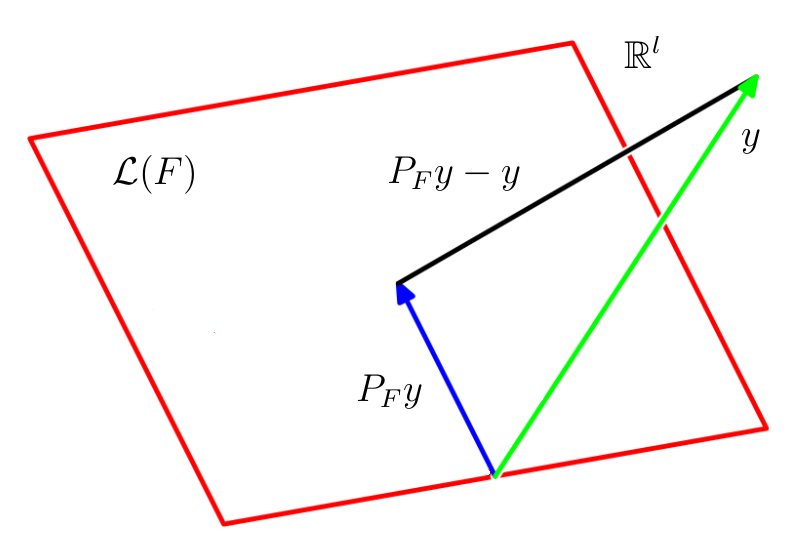
\includegraphics[height=200pt, keepaspectratio = true]{images/geometry}   
%	\end{figure}
%\end{frame}
%
%\begin{frame}\frametitle{Сингулярное разложение}
%	Произвольная $l \times n$-матрица представима в виде сингулярного разложения:\\
%	$$F = VDU^T$$\\
%	Основные свойства сингулярного разложения:\\
%	\begin{enumerate}[--]
%		\item $V_{l \times n} = (v_1, \dots, v_n)$ ортогональна, $V^TV = I_n$, \\столбцы $v_j$ - собственные векторы матрицы $FF^T$
%		\item $U_{n \times n} = (u_1, \dots, u_n)$ ортогональна, $U^TU = I_n$, \\столбцы $u_j$ - собственные векторы матрицы $F^TF$
%		\item $D$ диагональна, $D_{n \times n} = \operatorname{diag} (\sqrt{\lambda_1}, \dots, \sqrt{\lambda_n})$, \\$\lambda_j > 0$ - собственные значения матриц $F^TF$ и $FF^T$
%	\end{enumerate}
%\end{frame}
%
%\begin{frame}\frametitle{Решение МНК через сингулярное разложение}
%	Псевдообратная $F^+$, вектор МНК-решения $w^*$,
%	МНК-аппроксимация целевого вектора $Fw^*$\\
%	$F^+ = (UDV^TVDU^T)^{-1}UDV^T = UD^{-1}V^T = \sum\limits_{j=1}^n \frac{1}{\sqrt{\lambda_j}}  u_j v_j^T$\\
%	$ w^* = F^+y = UD^{-1}V^Ty = \sum\limits_{j=1}^n \frac{1}{\sqrt{\lambda_j}}  u_j (v_j^Ty)$\\
%	$F w^* = P_F y = (VDU^T)UD^{-1}V^Ty = VV^Ty = \sum\limits_{j=1}^n v_j (v_j^Ty)$\\
%	$\Vert w^* \Vert^2  = \Vert D^{-1}V^Ty \Vert^2 = \sum\limits_{j=1}^n \frac{1}{\lambda_j} (v_j^Ty)^2$
%\end{frame}
%
%\begin{frame}\frametitle{Проблема мультиколлинеарности}
%	Если $\exists \gamma \in \mathbb{R}^n: F\gamma \approx 0$, то некоторые $\lambda_j$ близки к нулю.\\
%	Число обусловленности $n \times n$-матрицы $F^TF = A$:
%	$$\mu(A) = \Vert A \Vert \Vert A^{-1} \Vert = \frac{\max\limits_{u: \Vert u \Vert = 1} \Vert A u \Vert}{\min\limits_{u: \Vert u \Vert = 1} \Vert A u \Vert} = \frac{\lambda_{max}}{\lambda_{min}}$$\\
%	При умножении обратной матрицы на вектор, $z = A^{-1}u$, относительная погрешность усиливается в $\mu(A)$ раз:\\
%	$$\frac{\Vert \delta z \Vert}{\Vert z \Vert } \leq \mu(A) \frac{\Vert \delta u \Vert}{\Vert u \Vert }$$
%\end{frame}
%
%\begin{frame}\frametitle{Проблема мультиколлинеарности}
%	Если матрица $F^TF$ плохо обусловлена, то: 
%	\begin{enumerate}[--]
%		\item решение становится неустойчивым и неинтерпретируемым, $\Vert w^* \Vert $ велико
%		\item на обучении $Q(w^*, X^l) = \Vert Fw^* -y \Vert$ -- мало   
%		\item на контроле $Q(w^*, X^k) = \Vert F'w^* -y' \Vert$ -- велико
%	\end{enumerate}
%	\alert{Вопрос:} Как бороться с этой проблемой?
%\end{frame}
%
%\begin{frame}\frametitle{Проблема мультиколлинеарности}
%	Стратегии устранения мультиколлинеарности и переобучения:
%	\begin{enumerate}[--]
%		\item Отбор признаков: $f_1, \dots, f_n \rightarrow f_{j_1}, \dots, f_{j_m}, \hspace{3mm} m << n$
%		\item Преобразование признаков: $f_1, \dots, f_n \rightarrow g_1, \dots, g_m,\hspace{3mm}  m << n$
%		\item Регуляризация: $\Vert w \Vert \rightarrow \min$
%	\end{enumerate}
%\end{frame}
%
%\begin{frame}\frametitle{Гребневая регрессия}
%	Штраф за увеличение нормы вектора весов $\Vert w \Vert$\\
%	$$Q_{\tau} (w) = \Vert F w - y \Vert^2 + \frac{1}{\sigma} \Vert w \Vert^2$$\\
%	где $\tau = \frac{1}{\sigma}$ -- неотрицательный параметр регуляризации.\\
%	\vspace{5mm}
%	Модифицированное МНК-решение ($\tau I_n$ — «гребень»)\\
%	$$w^*_{\tau} = (F^TF + \tau I_n)^{-1}F^Ty$$\\
%	
%	\textbf{Вопрос:} Можно ли подбирать $\tau$ не вычисляя каждый раз обратную матрицу?
%\end{frame}
%
%\begin{frame}\frametitle{Преимущество сингулярного разложения}
%	Модифицированное МНК-решение ($\tau I_n$ — «гребень»)\\
%	$$w^*_{\tau} = (F^TF + \tau I_n)^{-1}F^Ty$$\\
%	Преимущество сингулярного разложения:\\
%	можно подбирать параметр $\tau$ , вычислив сингулярное разложение только один раз.
%\end{frame}
%
%\begin{frame}\frametitle{Сингулярное разложение}
%	$$w_{\tau}^*= U(D^2 + \tau I_n)^{-1}DV^Ty = \sum\limits_{j=1}^n \frac{\sqrt{\lambda_j}}{\lambda_j + \tau} u_j(v_j^Ty)$$\\
%	$$Fw_{\tau}^* = VDU^Tw_{\tau}^* = V \operatorname{diag} \left(\frac{\lambda_j}{\lambda_j + \tau}\right) V^Ty = \sum\limits_{j=1}^n \frac{\lambda_j}{\lambda_j + \tau} v_j (v_j^Ty)$$\\
%	$$\Vert w_{\tau}^* \Vert^2 = \Vert U(D^2 + \tau I_n)^{-1} DV^T y \Vert^2 = \sum\limits_{j=1}^n \frac{\lambda_j}{(\lambda_j + \tau)^2} (v^T_j y)^2$$\\
%	$F w_{\tau}^* \neq Fw^*$ -- зато решение становится более устойчивым
%\end{frame}
%
%\begin{frame}\frametitle{Выбор параметра регуляризации $\tau$}
%	Контрольная выборка: $X^k = (x'_i, y'_i)_{i=1}^k$\\
%	%Вычисление функционала $Q$ на контрольных данных $T$ раз потребует $O(kn^2 + knT)$ операций:\\
%	$$Q(w_{\tau}^*,X^k) = \Vert F' w_{\tau}^* - y' \Vert^2 = \Vert F'U \operatorname{diag} \left(\frac{\lambda_j}{\lambda_j + \tau}\right) V^T y -y' \Vert^2$$\\
%	Зависимость $Q(\tau)$ обычно имеет характерный минимум.
%\end{frame}
%
%\begin{frame}\frametitle{Сокращение «эффективной размерности»}
%	Сокращение весов:\\
%	$$\Vert w_{\tau}^* \Vert^2 = \sum\limits_{j=1}^n \frac{\lambda_j}{(\lambda_j + \tau)^2} (v^T_j y)^2 < \Vert w^* \Vert^2  = \sum\limits_{j=1}^n \frac{1}{\lambda_j} (v_j^Ty)^2$$\\
%	Роль размерности играет след проекционной матрицы:\\
%	$$tr F(F^TF)^{-1}F^T = tr(F^TF)^{-1}F^TF = tr I_n = n$$\\
%	При использовании регуляризации:\\
%	$$tr F(F^TF + \tau I_n)^{-1}F^T = tr \hspace{1mm}  \operatorname{diag} \left(\frac{\lambda_j}{\lambda_j + \tau}\right)= \sum\limits_{j=1}^n \frac{\lambda_j}{\lambda_j + \tau } < n $$
%\end{frame}
%
%\begin{frame}\frametitle{LASSO}
%	LASSO -- Least Absolute Shrinkage and Selection Operator\\
%	$$
%	\begin{cases} Q(w,X^l) = \Vert Fw - y \Vert^2 \rightarrow \min\limits_{w} \\
%	\sum_{j=1}^n \vert w_j \vert \leq \kappa
%	\end{cases}
%	$$\\
%	После замены переменных:\\
%	$$
%	\begin{cases} w_j = w_j^+ - w_j^-\\
%	\vert w_j \vert = w_j^+ + w_j^-, \hspace{5mm} w_j^+, w_j^- \geq 0\\
%	
%	\end{cases}
%	$$\\
%	ограничения принимают канонический вид:\\
%	$$\sum\limits_{j=1}^n w_j^+ + w_j^- \leq \kappa$$\\
%	Чем меньше $\kappa$, тем больше $j$ таких, что $w_j^+ = w_j^- = 0$\\
%	%не гауссовское распределение, а лапласовское
%\end{frame}
%
%\begin{frame}\frametitle{Негладкие регуляризаторы}
%	Elastic Net:\\
%	$$\frac{1}{2} \Vert Fw - y \Vert^2 + \mu \sum\limits_{j=1}^n \vert w_j \vert + \frac{\tau}{2} \sum\limits_{j=1}^n w_j^2 \rightarrow \min\limits_{w}$$\\
%	Support Features Machine:\\
%	$$\frac{1}{2} \Vert Fw - y \Vert^2 + \tau \sum\limits_{j=1}^n R_{\mu}(w_j) \rightarrow \min\limits_{w}$$\\
%	$$ R_{\mu}(w_j) = \begin{cases} 2 \mu \vert w_j \vert, \hspace{2mm} \vert w_j \vert \leq \mu\\
%	\mu^2 + w_j^2, \hspace{2mm} \vert w_j \vert \geq \mu
%	\end{cases}$$\\
%	%Применение этих методов требует выбора траектории регуляризации в пространстве $(\mu, \tau )$
%\end{frame}

\end{document}